\documentclass[]{final_report}
\usepackage{graphicx}
\usepackage{hyperref}


%%%%%%%%%%%%%%%%%%%%%%
%%% Input project details
\def\studentname{Ciaran Palmer}
\def\projecttitle{SensorML on SenseTile}
\def\supervisorname{Your Supervisor Name}
\def\moderatorname{Your Moderator Name}


\begin{document}

\maketitle
\tableofcontents\pdfbookmark[0]{Table of Contents}{toc}\newpage

%%%%%%%%%%%%%%%%%%%%%%
%%% Your Abstract here

\begin{abstract}
SenseTileSensor Board

SensorML description.

WebServer to access sensor observations

SensorML Bon Mapping with a tool and method to develop sensorML descriptions

\end{abstract}




\newpage


%%%%%%%%%%%%%%%%%%%%%%
%%% Acknowledgments

\chapter*{Acknowledgments}


%%%%%%%%%%%%%%%%%%%%%%
%%% Introduction

\chapter{Introduction}

The aim of this thesis project was to model the SenseTile Sensor Board using Sensor Model Language (SensorML)\cite{SensoMLref} . A prototype of a Web Service for accessing SenseTile Sensor Board sensor observations was to be developed using this SensorML description of the SenseTile Sensor Board. An evaluation of the suitability of SensorML for use as part of the SenseTile System was also to be performed.

SenseTile is a sensor and processing package including motion sensors, RFID sensors, temperature sensor, audio sensors, pressure sensors, light level sensors video sensors among others. It is used as a replacement for standard ceiling tiles to provide smart building services as part of a Web Sensor Network. The SenseTile System is made up of two units a Sensor Board and Processor Unit. The sensors are interfaced or hosted on the Sensor Board. The Processor Unit interfaces to the Sensor Board allowing data from the Sensor Board to be processed futher as required.

SensorML was developed to describe sensor systems and the processing of sensor observations. It provides standard models and XML encodings to describe the process of sensor measurement. SensorML is one of a suite of specifications provided by the Open Geospatial Consortium (OGC) as part of the Sensor Web Enablement(SWE) initiative[ref]. The members of the OGC have the goal of developing open standards to exploit Web connected sensors of all types.

The SenseTile Web Service allows access to the Sensor Board sensor observations and SensorML description. It would run on the SenseTile Processor Unit.  The Web Service is based on another OGC SWE  specification, the Sensor Observation Service (SOS)[ref]. This specification defines a standard Web interface for retrieving information about sensor systems and sensor observations. Sensor Board measurements that have been post processed and converted to real values or the raw Sensor Board data can be accessed using the Web Service.

SensorML and SOS specification depend on another SWE specification, Observation and Measurements(O\&M)[ref]. This specification provides standard models and XML encoding for sensor observations.SWE Common - common data models and schema

A  SensorML to BON Mapping was also to be explored . BON\cite{BONref} is a notation and a method for Object Oriented systems analysis and design. Based on this mapping it was proposed to develop a tool/method to automatically generate SensorML descriptions. Generally SensorML is hand generated with all the shortcomings of such an approach. The proposed approach would allow sensor processing to defined formally in BON and then refined to JML/Java. 


\chapter{ Background Research}



\section{Sensor Networks and SWE}
How was problem solved before.


\section{SensorML}
The Open Geospatial Consortium (OGC) Sensor Web Enablement (SWE) [ref]  is establishing interfaces and protocols that will enable a standardised “Sensor Web”. It is hoped that an easier integration and development of sensor applications across sensor networks will be facilitated by this standarising activity. Sensor Modelling Language (SensorML) is one part of the SWE initiative and is used to describe sensor systems and the processing of observations from sensor systems.

The purposes of SensorML are to:
• Provide descriptions of sensors and sensor systems for inventory management
• Provide sensor and process information in support of resource and observation discovery
• Support the processing and analysis of the sensor observations
• Support the geolocation of observed values (measured data)
• Provide performance characteristics (e.g., accuracy, threshold, etc.)
• Provide an explicit description of the process by which an observation was obtained (i.e., it’s lineage)
• Provide an executable process chain for deriving new data products on demand (i.e., derivable observation)
• Archive fundamental properties and assumptions regarding sensor systems

SensorML provides a functional model of sensors and an XML encoding to describe sensors and their observations.
Sensors are modelled as processes that convert real phenomena to data. Processes take inputs, process them and result in one or several outputs. They can also define relevant metadata. The processes can be connected together in chains using SensorML ProcessChains or Systems. 

including measurement by a sensor system, as well as post-measurement
processing.

When Modelling a sensor system in SensorML the main entities used are Systems and Components. A SensorML System is used to group sensors that are related spatially to one another.  A Component is an atomic process that generally converts a physical phenomen to a digital number. ProcessModels are another modelling that is used to describe a pure process that has no physicality

Quantity, Count, Boolean, Category, and Time provide the basic primitives. Within SensorML, these serve as the basis for specifying all inputs, outputs, and parameters within a Process

DataRecord or DataArray.

Detector model.

The SensorML description of the SenseTile Sensor Board is shown in the following section.
\section{BON}
\section{SOS}
\section{OGC Lib}


\chapter{Design}
\section{SensorML Description of SenseTile}

SensorML System and Component were used to describe the SenseTile system and it's sensors. The sensor specifications were used to generate the metadata.
The Sensors are modelled a detectors. They are process that take scalar values
and can perform transformations on them.

System is providing the mapping of inputs to processes and the outputs.

Naming rules inputs and outputs - allow more generic handling of implementation classes.

Processed verus raw data.

It is further recognized that most sensor observations consist of at least two processes: a sampling process and a conversion process.

 \begin{figure}
\scalebox{0.65}{\includegraphics{SenseTileSystem.pdf}}
\caption{SenseTile System Overview}\label{fig:SenseTileSystem.pdf}
\end{figure}

 \begin{figure}
\scalebox{0.65}{\includegraphics{SensorML_SenseTile_System_2_pa1.pdf}}
\caption{SenseTile System Components}\label{fig:SensorML_SenseTile_System_2_pa1.pdf}
\end{figure}

\subsection{SenseTile System}
\subsection{Light Sensor}
\subsection{Thermistor}
\subsection{Pressure Sensor}
\subsection{Accelerometer}
\subsection{Acoustic Sensor}

Types
 - SWE -

Count - BigInteger
Quantity - Double

DataArray

 * Carries an array of int primitives.
 * All data is casted to other types when requested.


\newpage
\section{BON to SensorML mapping}
Features to be elements or attributes.

Name rule suffix "Attrib" to make it an attribute.

List handling - convention for mapping.

SML prefix to handled key word clashes between sensorML and BON.

How to display this in thesis?
\section{SenseTile Web Service}
\subsection{Overview}

Web Service - SOS -standard access to sensor observations
The Sensor Observation Service (SOS) is an approved Open Geospatial Consortium standard. The standard defines a web service interface for the discovery and retrieval of real time or archived data produced by all kinds of sensors like mobile or stationary as well as in-situ or remote sensors.

The sensor data can be either observations or descriptions of the producing sensors containing metadata like calibration information, positions, etc. Observations are returned encoded as OM Observations, while information about sensors are returned encoded in SensorML or TML. Used in conjunction with these OGC standards and other OGC specifications, the SOS provides a broad range of interoperable capability for discovering, binding to and interrogating individual sensors, sensor platforms, or networked constellations of sensors in real-time, archived or simulated environments. 
SOS diagram

DataProvider

DataProducer

Deployment Scenarios - diagram

Flexible Division - several dataproducers can register with one DataProvider.

Seperate processes rmi.
 \begin{figure}
\scalebox{0.65}{\includegraphics{SystemOverview.png}}
\caption{Overview}\label{fig:SystemOverview.png}
\end{figure}


 \begin{figure}
\scalebox{0.65}{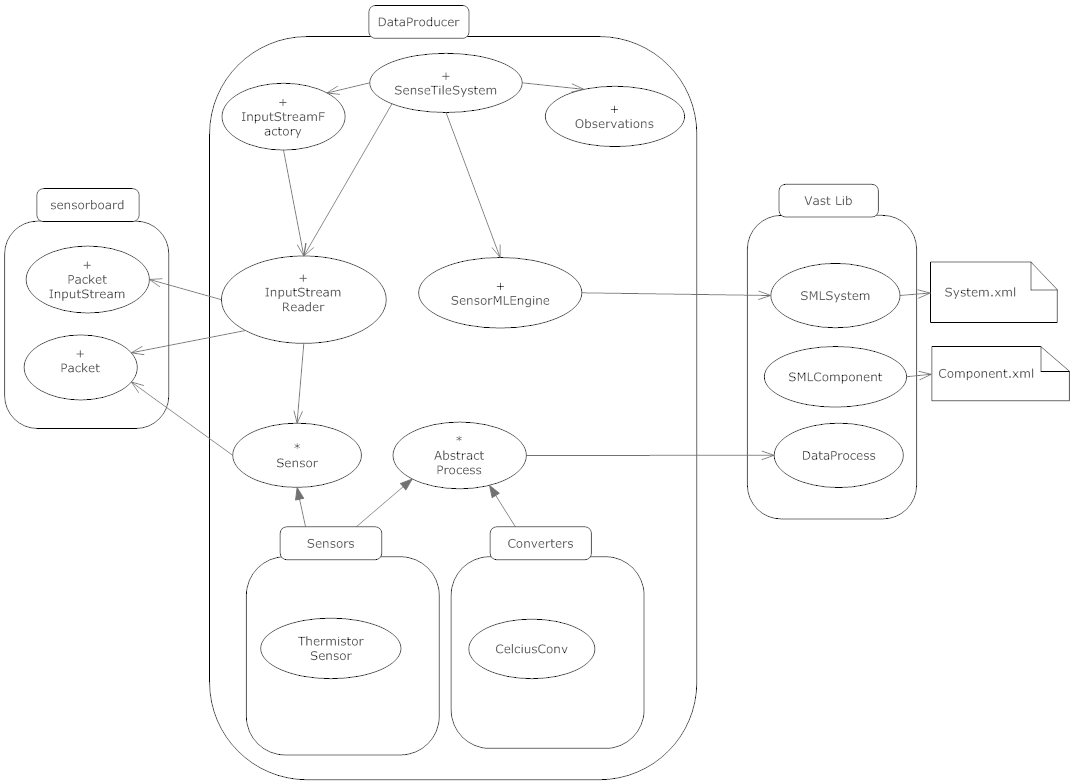
\includegraphics{sensetile_static_diagam.png}}
\caption{DataProducer Static Diagram}\label{fig:sensetile_static_diagam.png}
\end{figure}

\subsection{DataProducer}
Use PacketInput stream to access SenseTile observation packets.

System reads packets and averages them for every configurable seconds. Default 1.

Thermistor components reads out the temperature value
and its output is sent to both the raw data and the celcius
converter component and on to the tuples.

These tuples are sent to webservice provider as observations.

Observation as described in SOS.

\subsection {DataProvider}
 \begin{figure}
\scalebox{0.65}{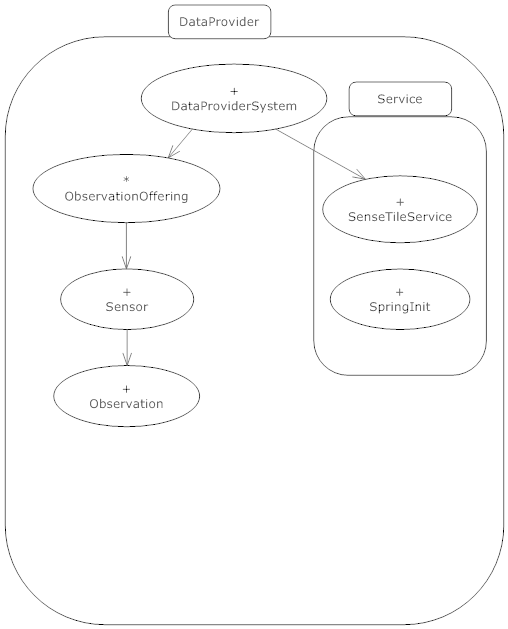
\includegraphics{bon_static_diagam_provider.png}}
\caption{DataProvider Static Diagram}\label{fig:bon_static_diagam_provider.png}
\end{figure}
Keeps track of sensorboards that register

provides an RMI interface to the DataProducer to update with observations. 


GetObservaton - marshal Observation to xml string and send as response.

StreamObservation -  registered clients get new observation sent over UDP connection?

Provides a Web Service interface  based on Sensor Observation Service. Not fully as is a very complex interface.

\newpage
\section{SensorML generation}

Java binding wth JIBX  generate sensorml.

Simple xml file with Sensor metadata.

Naming rules allow connection of inputs and outputs
in sensorML processes.

 component id +Input

 component id+Output

\chapter{ Detailed Design and Implementation}

\section{SenseTile WebService}

DataProvider is based on AXIS 2.0/Spring

DataProducer POJO/VastLib/UCD SenseTile Driver Lib

RMI used between DataProvider and DataProducer.

\section{SensorML Generation}

\chapter{Results}

Tested against real SenseTile and sensor data retrieved by a testclient.

Generation of SensorML description of a Senstile Sensor

\chapter{ Conclusions and Future Work}

what has been achieved
the weaknesses of your approach

\chapter{References}
\newpage
\begin{thebibliography}{99}
\bibitem{SensoMLref}Open Geospatial Consortium Inc., OpenGIS Sensor Model Language (SensorML) Implementation Specification, 2007
\bibitem{SOSref}Open Geospatial Consortium Inc., OpenGIS  Implementation Specification, 2007
\bibitem{OMref}Open Geospatial Consortium Inc., OpenGIS  Implementation Specification, 2007
\bibitem{SWEArchref}Open Geospatial Consortium Inc., , 2007
\bibitem{SMLTutorialref}Open Geospatial Consortium Inc., , 2007


\bibitem{BONref}Kim Waldén and Jean-Marc Nerson , "Seamless Object-Oriented Software Architecture", 1995
\end{thebibliography}
\label{endpage}


\chapter{Appendices}






\end{document}

\end{article}
